\documentclass[handout]{beamer}  
%use [handout] option to print without all the pauses!
\usepackage{setspace}
\linespread{1.3}
\usepackage{amssymb, amsmath, amsthm} 
\usepackage{rotating}
\usepackage{multirow}
\usepackage{graphicx}
\usepackage{enumerate}
\usepackage{synttree}
\usepackage{fancybox}
\usepackage{color}
\usepackage{tikz}
\usetikzlibrary{trees}
\newcommand{\p}{\mathbb{P}}
\newcommand{\expect}{\mathbb{E}}
\newcommand{\var}{\mathbb{V}}



%\setbeamertemplate{blocks}[rounded][shadow=true] 
%gets rid of bottom navigation bars
\setbeamertemplate{footline}{
   \begin{beamercolorbox}[ht=4ex,leftskip=0.3cm,rightskip=0.3cm]{author in head/foot}
%    \usebeamercolor{UniBlue}
    \vspace{0.1cm}
    %\insertshorttitle \ - \insertdate 
    \hfill \insertframenumber / 
    \inserttotalframenumber
   \end{beamercolorbox}
   \vspace*{0.1cm}
} 

%gets rid of navigation symbols
\setbeamertemplate{navigation symbols}{}


%Include or exclude the notes?
%\setbeameroption{show notes}
\setbeameroption{hide notes}


\title[Econ 103]{Economics 103, Statistics for Economists} 
\author[F. DiTraglia]{Francis J.\ DiTraglia}
\institute{University of Pennsylvania}
\date{Lecture 20}


\begin{document} 




%%%%%%%%%%%%%%%%%%%%%%%%%%%%%%%%%%%%%%%%

\begin{frame}[plain]
	\titlepage 
	

\end{frame} 


%%%%%%%%%%%%%%%%%%%%%%%%%%%%%%%%%%%%%%%%
\begin{frame}
\begin{center}
\Huge Hypothesis Testing I
\end{center}
\end{frame}

%%%%%%%%%%%%%%%%%%%%%%%%%%%%%%%%%%%%%%%%
\begin{frame}
\frametitle{An excerpt from \emph{The Lady Tasting Tea} by David Salsburg}
\footnotesize
\begin{quote}
It was a summer afternoon in Cambridge, England, in the late 1920s. A group of university dons, their wives, and some guests were sitting around an outdoor table for afternoon tea. One of the women was insisting that tea tasted different depending upon whether the tea was poured into the milk or whether the milk was poured into the tea. The scientific minds among the men scoffed at this as sheer nonsense. What could be the difference? They could not conceive of any difference in the chemistry of the mixtures that could exist. A thin, short man, with thick glasses and a Vandyke beard beginning to turn gray, pounced on the problem. ``Let us test the proposition'' he said excitedly. He began to outline an experiment in which the lady who insisted there was a diference would be presented with a sequence of cups of tea, in some of which the milk had been poured into the tea and in others of which the tea had been poured into the milk.
\end{quote}
\end{frame}
%%%%%%%%%%%%%%%%%%%%%%%%%%%%%%%%%%%%%%%%
% \begin{frame}

% \begin{figure}
% 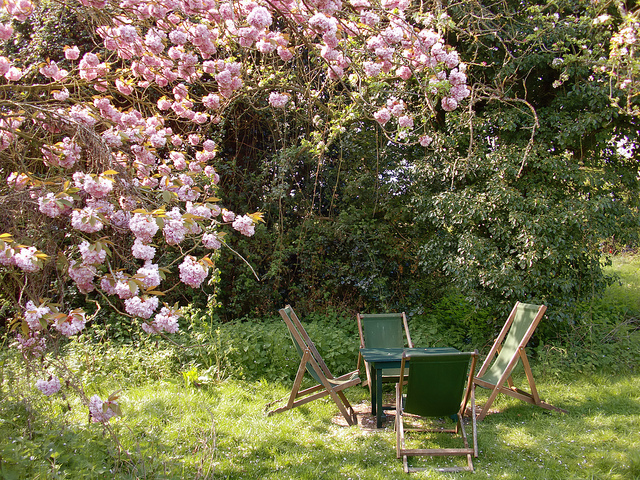
\includegraphics[scale = 0.35]{./images/grant1}

% \caption{The Orchard, Grantchester}
% \end{figure}

% \end{frame}

% %%%%%%%%%%%%%%%%%%%%%%%%%%%%%%%%%%%%%%%%
% \begin{frame}

% \begin{figure}
% 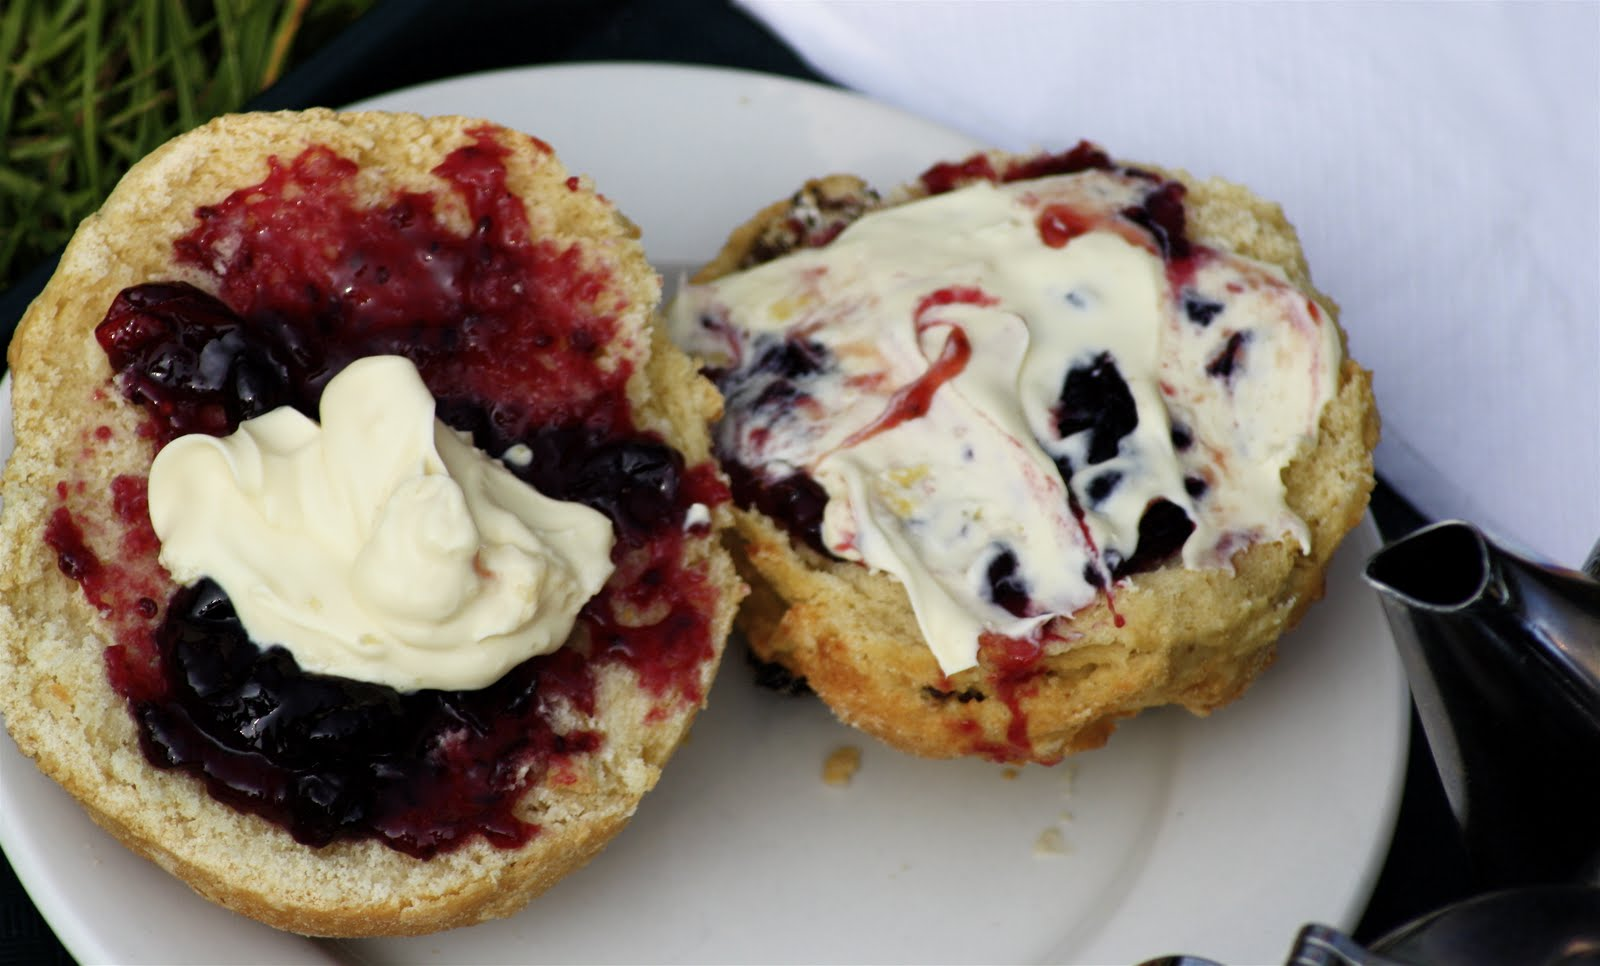
\includegraphics[scale = 0.15]{./images/grant2}

% \caption{What to have with your tea.}
% \end{figure}

% \end{frame}

% %%%%%%%%%%%%%%%%%%%%%%%%%%%%%%%%%%%%%%%%

% \begin{frame}

% \begin{figure}
% 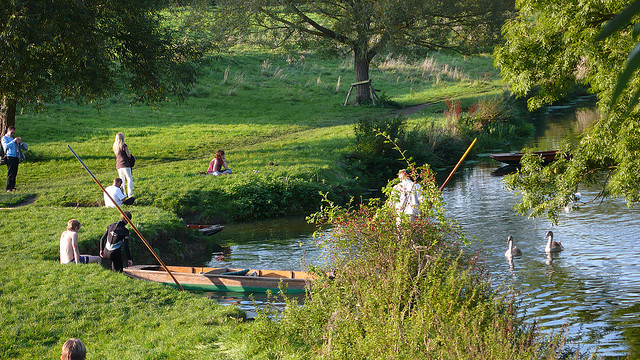
\includegraphics[scale = 0.31]{./images/grant6}\\
% \vspace{0.6em}
% 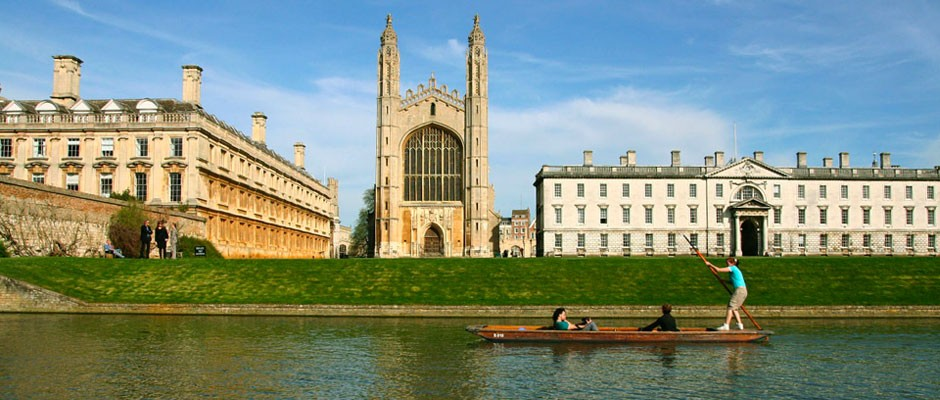
\includegraphics[scale = 0.211]{./images/grant7}

% \caption{Why walk when you can punt?}
% \end{figure}

% \end{frame}

% %%%%%%%%%%%%%%%%%%%%%%%%%%%%%%%%%%%%%%%%
% \begin{frame}

% \begin{figure}
% 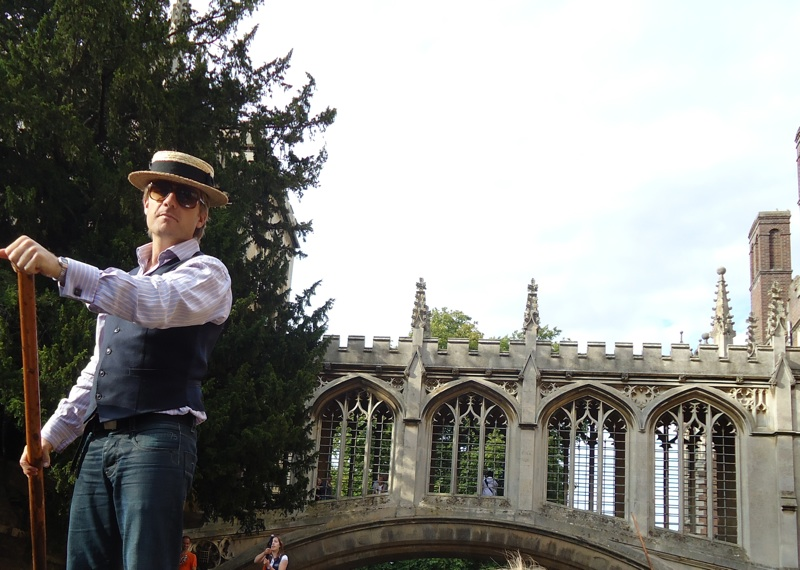
\includegraphics[scale = 0.3]{./images/grant8}

% \caption{What to wear. (Yes, I do in fact own such a hat.)}
% \end{figure}

% \end{frame}

% %%%%%%%%%%%%%%%%%%%%%%%%%%%%%%%%%%%%%%%%
\begin{frame}
\frametitle{Continued...}
\footnotesize
\begin{quote}
And so it was that summer afternoon in Cambridge. The man with the Vandyke beard was Ronald Aylmer Fisher, who was in his late thirties at the time. He would later be knighted Sir Ronald Fisher. In 1935, he wrote a book entitled The Design of Experiments, and he described the experiment of the lady tasting tea in the second chapter of that book. In his book, Fisher discusses the lady and her belief as a hypothetical problem. He considers the various ways in which an experiment might be designed to determine if she could tell the difference.
\end{quote}
\end{frame}

%%%%%%%%%%%%%%%%%%%%%%%%%%%%%%%%%%%%%%%%
\begin{frame}
\begin{center}
\Huge The Pepsi Challenge \\
	\large (Volunteers: 1 ``Expert,'' 1 Skeptic)
\end{center}
\end{frame}
%%%%%%%%%%%%%%%%%%%%%%%%%%%%%%%%%%%%%%%%
\begin{frame}
\frametitle{The Pepsi Challenge}
Our expert claims to be able to tell the difference between Coke and Pepsi. Let's put this to the test! 
\begin{itemize}
\item Eight cups of soda 
	\begin{itemize}
\item Four contain Coke 
\item Four contain Pepsi 
\end{itemize}
	\item The cups are randomly arranged 
	\item How can we use this experiment to tell if our expert can \emph{\alert{really}} tell the difference?
\end{itemize}
\end{frame}
%%%%%%%%%%%%%%%%%%%%%%%%%%%%%%%%%%%%%%%%
\begin{frame}
\frametitle{The Results:}
	\# of Cokes Correctly Identified: \\ \vspace{2em}
	\alert{What do you think? Can our expert really tell the difference? 
\includegraphics[scale = 0.05]{./images/clicker}}
		\begin{enumerate}[(a)]
\item Yes
\item No
\end{enumerate}
\end{frame}

%%%%%%%%%%%%%%%%%%%%%%%%%%%%%%%%%%%%%%%%
\begin{frame}
\frametitle{
\includegraphics[scale = 0.05]{./images/clicker}}
If you just guess randomly, what is the probability of identifying \emph{all four cups of Coke correctly}?
\pause
\begin{itemize}
\item ${8\choose 4}=70$ ways to choose four of the eight cups. \pause
\item If guessing randomly, each of these is \emph{\alert{equally likely}} \pause
\item Only \emph{\alert{one}} of the 70 possibilities corresponds to correctly \pause identifying all four cups of Coke. \pause
\item Thus, the probability is $1/70 \approx 0.014$
\end{itemize}
\end{frame}
%%%%%%%%%%%%%%%%%%%%%%%%%%%%%%%%%%%%%%%%
\begin{frame}
\frametitle{
\includegraphics[scale = 0.05]{./images/clicker}}
If you just guess randomly, what is the probability of identifying \emph{all but one cup of Coke correctly}?
\pause
\begin{itemize}
\item ${8\choose 4}=70$ ways to choose four of the eight cups. \pause
\item If guessing randomly, each of these is \emph{\alert{equally likely}} \pause
\item There are 16 ways to mis-identify one Coke: 
	\begin{itemize}
		\item $4$ choices of \emph{which} Coke you call a Pepsi 
		\item $4$ choices of \emph{which} Pepsi you call a Coke 
		\item Total of $4\times 4 = 16$ possibilities \pause
	\end{itemize}	
\item Thus, the probability is $16/70 \approx 0.23$
\end{itemize}
\end{frame}
%%%%%%%%%%%%%%%%%%%%%%%%%%%%%%%%%%%%%%%%
\begin{frame}
\frametitle{Probabilities if Guessing Randomly}
	\begin{center}
		\begin{tabular}{rccccc}
		\hline
		\# Correct & 0 & 1 & 2 & 3 & 4\\
		Prob.&1/70 & 16/70 & 36/70 & 16/70 &1/70\\
		\hline
		\end{tabular}
	\end{center}
\end{frame}
%%%%%%%%%%%%%%%%%%%%%%%%%%%%%%%%%%%%%%%%
\begin{frame}
	\frametitle{
\includegraphics[scale = 0.05]{./images/clicker}}
	\begin{center}
		\begin{tabular}{rccccc}
		\hline
		\# Correct & 0 & 1 & 2 & 3 & 4\\
		Prob.&1/70 & 16/70 & 36/70 & 16/70 &1/70\\
		\hline
		\end{tabular}
	\end{center}
	If you're just guessing, what is the probability of identifying \alert{\emph{at least}} three Cokes correctly?
	\pause
	\begin{itemize}
\item Probabilities of mutually exclusive events sum. 
\item $P$(all four correct) = 1/70 
\item $P$(exactly 3 correct )= 16/70 
\item $P$(at least three correct) $ = 17/70 \approx 0.24$

\end{itemize}
\end{frame}

%%%%%%%%%%%%%%%%%%%%%%%%%%%%%%%%%%%%%%%%
\begin{frame}
\frametitle{The Pepsi Challenge}
	\begin{itemize}
\item Even if you're just guessing randomly, the probability of correctly identifying three or more Cokes is around 24\% 
\item In contrast, the probability of identifying \emph{\alert{all four}} Cokes correctly is only around 1.4\% if you're guessing randomly. 
\item We should probably require the expert to get them all right. 
\item What if the expert gets them all wrong? This also has probability $1.4\%$ if you're guessing randomly...
\end{itemize}
\end{frame}

%%%%%%%%%%%%%%%%%%%%%%%%%%%%%%%%%%%%%%%%

\begin{frame}
	\begin{center}
	\huge That was a Hypothesis Test!\\
	\normalsize We'll go through the details in a moment, but first an analogy...
	\end{center}
\end{frame}

%%%%%%%%%%%%%%%%%%%%%%%%%%%%%%%%%%%%%%%%



\begin{frame}
	\begin{center}
	\huge Hypothesis Testing is Similar to a Criminal Trial
	\end{center}
\end{frame}

%%%%%%%%%%%%%%%%%%%%%%%%%%%%%%%%%%%%%%%%

\begin{frame}
%\frametitle{Hypothesis Testing -- Analogy to Criminal Trial}
\footnotesize
\begin{columns}
\begin{column}[l]{6cm} 
 %FIRST COLUMN HERE
   	\begin{block}{Criminal Trial}
	\begin{itemize}
		\item<1-> The person on trial is either innocent or guilty (but not both!)
		\item<2-> ``Innocent Until Proven Guilty''
		\item<3-> Only convict if evidence is ``beyond a shadow of a doubt''
		\item<4-> \emph{Not Guilty} rather than Innocent
			\begin{itemize}\footnotesize
				\item<5-> Acquit $\neq$ Innocent
			\end{itemize}
		\item<6-> Two Kinds of Errors:
			\begin{itemize} \footnotesize
				\item<6-> Convict the innocent
				\item<6->  Acquit the guilty
			\end{itemize}
		\item<7-> Convicting the innocent is a worse error. Want this to be rare even if it means acquitting the guilty.	\end{itemize}
\end{block}
   
   
\end{column} 
\begin{column}[l]{6cm} 

 %SECOND COLUMN HERE 

\begin{block}{Hypothesis Testing}
		\begin{itemize}
		\item<1-> Either the null hypothesis $H_0$ or the alternative $H_1$  hypothesis is true.
		\item<2-> Assume $H_0$ to start
		\item<3-> Only reject $H_0$ in favor of $H_1$ if there is strong evidence.
		\item<4-> \emph{Fail to reject} rather than Accept $H_0$	
		\begin{itemize} \footnotesize
			\item<5-> (Fail to reject $H_0) \neq (H_0$ True) 
		\end{itemize}
				\item<6-> Two Kinds of Errors:
			\begin{itemize} \footnotesize
				\item<6-> Reject true $H_0$ (Type I)
				\item<6-> Don't reject false $H_0$ (Type II)
			\end{itemize}
			\item<7-> Type I errors (reject true $H_0$) are worse: make them rare even if that means more Type II errors.
	\end{itemize}
\end{block}

\end{column} 
\end{columns} 

\end{frame}
%%%%%%%%%%%%%%%%%%%%%%%%%%%%%%%%%%%%%%%%
\begin{frame}
\frametitle{How is the Pepsi Challenge a Hypothesis Test?}
	\begin{block}{Null Hypothesis $H_0$}
		Can't tell the difference between Coke and Pepsi: just guessing. \pause
\end{block}
	\begin{block}{Alternative Hypothesis $H_1$}
	Able to distinguish Coke from Pepsi.\pause
\end{block}
	\begin{block}{Type I Error -- Reject $H_0$ even though it's true} 
	Decide expert can tell the difference when she's really just guessing. \pause
\end{block}
	\begin{block}{Type II Error -- Fail to reject $H_0$ even though it's false}
	Decide expert just guessing when she really can tell the difference. 
\end{block}
\end{frame}
%%%%%%%%%%%%%%%%%%%%%%%%%%%%%%%%%%%%%%%%
\begin{frame}
\frametitle{How do we find evidence to reject $H_0$?}
	\begin{itemize}
		\item Choose a \alert{significance level $\alpha$} maximum probability of Type I error that we are willing to tolerate. 
			\begin{itemize}
				\item Measures how often we will reject a true null, i.e.\ convict an innocent person \pause
			\end{itemize}
		\item Test Statistic $T_n$ uses sample to measure plausibility of $H_0$ \pause
		\item Null Hypothesis $H_0 \Rightarrow$ Sampling Distribution for $T_n$  
			\begin{itemize}
				\item ``Under the null'' means ``assuming the $H_0$ is true'' \pause
			\end{itemize}
		\item Using $\alpha$ and the sampling distribution of $T_n$ under the null, we construct a \alert{decision rule} in terms of a critical value $c_\alpha$ \pause
			\begin{itemize}
				\item Reject $H_0$ if $T_n > c_\alpha$
			\end{itemize}
	\end{itemize}
	
\end{frame}
%%%%%%%%%%%%%%%%%%%%%%%%%%%%%%%%%%%%%%%%
% \begin{frame}
% \frametitle{We still have a random sampling model in mind!}
% \footnotesize
% \begin{block}{Why does $T_n$ have a sampling distribution?}
% 	\begin{itemize}
% 		\item Random Sampling: new data $\Rightarrow$ different \emph{realization} $t$ of $T_n$ 
% 		\item Key point: $T_n$ is a \emph{random variable} with a particular distribution under the null hypothesis $H_0$ \pause
% 	\end{itemize}
% \end{block}

% \begin{block}{What do we mean by $\alpha$?} 
% 	\begin{itemize}
% 		\item $T_n$ is a RV $\Rightarrow$ outcome of hypothesis test is random! 
% 		\item Sometimes we make mistake: either reject $H_0$ when it is true or fail to reject it when it is false. 
% 		\item Repeated Sampling $\Rightarrow$ many different realizations of $T_n\Rightarrow$ many different outcomes of the test. 
% 		\item Test is constructed so that, if $H_0$ is true, we will reject it no more than $100\times \alpha \%$ of the time under repeated sampling.
% 	\end{itemize}
% \end{block}
% \end{frame}


%%%%%%%%%%%%%%%%%%%%%%%%%%%%%%%%%%%%%%%%
\begin{frame}
\frametitle{Example: Pepsi Challenge}
	\begin{block}{Test Statistic $T_n$}
		$T_n =$ Number of Cokes correctly identified
\end{block} 
	\begin{block}{$H_0\colon$ No skill, just guessing randomly}
	Under this null hypothesis, the sampling distribution of $T_n$ is:
		\begin{center}
		\begin{tabular}{rccccc}
		\hline
		\# Correct & 0 & 1 & 2 & 3 & 4\\
		Prob.&1/70 & 16/70 & 36/70 & 16/70 &1/70\\
		\hline
		\end{tabular}
	\end{center}
\end{block}


\end{frame}
%%%%%%%%%%%%%%%%%%%%%%%%%%%%%%%%%%%%%%%%
\begin{frame}
\frametitle{Example: Pepsi Challenge \hfill 
\includegraphics[scale = 0.05]{./images/clicker}}
$T_n\colon$ \# of Cokes correctly identified. Sampling Dist.\ under $H_0$:
		\begin{center}
		\begin{tabular}{rccccc}
		\hline
		\# Correct & 0 & 1 & 2 & 3 & 4\\
		Prob.&1/70 & 16/70 & 36/70 & 16/70 &1/70\\
		\hline
		\end{tabular}
	\end{center}
	\alert{If I choose a significance level of $\alpha =0.05$, what critical value should I use?}\\ (Remember that $\alpha$ is the probability of rejecting $H_0$ when it is actually true.)
	\pause
	
	\vspace{2em}
	Want $P(\mbox{Reject } H_0|H_0 \mbox{ True})\leq 0.05$\\ \pause
	$P(T_n \geq 3 |\mbox{Just Guessing}) = 17/70 \approx 0.23 > 0.05$ \pause
	$P(T_n \geq 4 |\mbox{Just Guessing}) = 1/70 \approx 0.014 \alert{\leq 0.05}$ 
\end{frame}
%%%%%%%%%%%%%%%%%%%%%%%%%%%%%%%%%%%%%%%%
\begin{frame}
\frametitle{Example: Pepsi Challenge \hfill 
\includegraphics[scale = 0.05]{./images/clicker}}
$T_n\colon$ \# of Cokes correctly identified. Sampling Dist.\ under $H_0$:
		\begin{center}
		\begin{tabular}{rccccc}
		\hline
		\# Correct & 0 & 1 & 2 & 3 & 4\\
		Prob.&1/70 & 16/70 & 36/70 & 16/70 &1/70\\
		\hline
		\end{tabular}
	\end{center}
	\alert{If I choose a significance level of $\alpha =0.25$, what critical value should I use?}
	\pause
	
	\vspace{2em}
	Want $P(\mbox{Reject } H_0|H_0 \mbox{ True})\leq 0.25$\\ \pause
	$P(T_n \geq 2 |\mbox{Just Guessing}) = 53/70 \approx 0.76 > 0.25$  \pause
	$P(T_n \geq 3 |\mbox{Just Guessing}) = 17/70 \approx 0.23 \alert{\leq 0.25}$ 
\end{frame}
%%%%%%%%%%%%%%%%%%%%%%%%%%%%%%%%%%%%%%%%



%%%%%%%%%%%%%%%%%%%%%%%%%%%%%%%%%%%%%%%%
\begin{frame}
\frametitle{Example: Pepsi Challenge \hfill 
\includegraphics[scale = 0.05]{./images/clicker}}
\footnotesize 
$H_0\colon$ Expert is just guessing randomly.\\
$H_1\colon$ Expert can distinguish Coke from Pepsi.\\
$T_n\colon$ \# of Cokes correctly identified. Has following sampling under the null:
		\begin{center}
		\begin{tabular}{rccccc}
		\hline \footnotesize
		\# Correct & 0 & 1 & 2 & 3 & 4\\
		Prob.&1/70 & 16/70 & 36/70 & 16/70 &1/70\\
		\hline
		\end{tabular}
	\end{center}
	\vspace{2em}
	\normalsize
	\alert{If I choose $\alpha =0.05$, what decision rule should I use?}
	\begin{enumerate}[(a)]
		\item Reject $H_0$ if $T_n \geq 0$
		\item Reject $H_0$ if $T_n \geq 1$
		\item Reject $H_0$ if $T_n \geq 2$
		\item Reject $H_0$ if $T_n \geq 3$
		\item Reject $H_0$ if $T_n \geq 4$
	\end{enumerate}
\end{frame}
%%%%%%%%%%%%%%%%%%%%%%%%%%%%%%%%%%%%%%%%
\begin{frame}
\frametitle{Example: Pepsi Challenge \hfill 
\includegraphics[scale = 0.05]{./images/clicker}}
\footnotesize 
$H_0\colon$ Expert is just guessing randomly.\\
$H_1\colon$ Expert can distinguish Coke from Pepsi.\\
$T_n\colon$ \# of Cokes correctly identified. Has following sampling under the null:
		\begin{center}
		\begin{tabular}{rccccc}
		\hline \footnotesize
		\# Correct & 0 & 1 & 2 & 3 & 4\\
		Prob.&1/70 & 16/70 & 36/70 & 16/70 &1/70\\
		\hline
		\end{tabular}
	\end{center}
	\vspace{2em}
	\normalsize
	\alert{If I choose $\alpha =0.05$, what decision rule should I use?}\\
\vspace{1em}
	Need $P(\mbox{Reject } H_0|H_0 \mbox{ True})\leq \alpha = 0.05$ \pause
	\begin{eqnarray*}
		P(T_n \geq 3 |\mbox{Just Guessing}) &=& 17/70 \pause \approx 0.23 > 0.05 \\\pause
	P(T_n \geq 4 |\mbox{Just Guessing}) &=& 1/70 \pause \approx 0.014 \alert{\leq 0.05}
	\end{eqnarray*}
	\vspace{1em}\pause
	\alert{Critical value for $\alpha = 0.05$ is 4}
\end{frame}
%%%%%%%%%%%%%%%%%%%%%%%%%%%%%%%%%%%%%%%%

\begin{frame}
\frametitle{Example: Pepsi Challenge \hfill 
\includegraphics[scale = 0.05]{./images/clicker}}
\footnotesize 
$H_0\colon$ Expert is just guessing randomly.\\
$H_1\colon$ Expert can distinguish Coke from Pepsi.\\
$T_n\colon$ \# of Cokes correctly identified. Has following sampling under the null:
		\begin{center}
		\begin{tabular}{rccccc}
		\hline \footnotesize
		\# Correct & 0 & 1 & 2 & 3 & 4\\
		Prob.&1/70 & 16/70 & 36/70 & 16/70 &1/70\\
		\hline
		\end{tabular}
	\end{center}
	\vspace{2em}
	\normalsize
	\alert{If I choose $\alpha =0.25$, what critical value should I use?}
	\begin{enumerate}[(a)]
		\item 0
		\item 1
		\item 2
		\item 3
		\item 4
	\end{enumerate}
\end{frame}
%%%%%%%%%%%%%%%%%%%%%%%%%%%%%%%%%%%%%%%%
\begin{frame}
At what significance levels would we reject the assumption that our expert was guessing randomly?
\end{frame}
%%%%%%%%%%%%%%%%%%%%%%%%%%%%%%%%%%%%%%%%

\begin{frame}
\frametitle{P-values}
Reject or fail to reject at a given significance level is a somewhat crude: doesn't tell us whether it was ``close'' or ``no contest.'' P-value is more informative: \pause
	\begin{block}{P-Value = Strength of evidence against the null}
	The p-value for a hypothesis test is the probability that we would observe a test statistic \emph{at least as extreme} as the one actually observed \emph{if the null hypothesis were true}.
\end{block}
\pause
\vspace{1em}
\alert{This means that the p-value equals the \emph{smallest significance level} at which our observed test statistic would cause us to reject $H_0$. It may be tempting to conclude that a p-value is the probability that the null is false but this is NOT CORRECT.}
\end{frame}

\begin{frame}
\frametitle{Example: Pepsi Challenge \hfill 
\includegraphics[scale = 0.05]{./images/clicker}}
\footnotesize 
$H_0\colon$ Expert is just guessing randomly.\\
$H_1\colon$ Expert can distinguish Coke from Pepsi.\\
$T_n\colon$ \# of Cokes correctly identified. Has following sampling under the null:
		\begin{center}
		\begin{tabular}{rccccc}
		\hline \footnotesize
		\# Correct & 0 & 1 & 2 & 3 & 4\\
		Prob.&1/70 & 16/70 & 36/70 & 16/70 &1/70\\
		\hline
		\end{tabular}
	\end{center}
	\vspace{2em}
	\normalsize
	\alert{Our observed test statistic was $\boxed{2}$ since the expert correctly identified this many Cokes. What is the p-value in this case?}\pause
	\begin{eqnarray*}
		P(T_n \geq \alert{\boxed{2}}|H_0 \mbox{ True}) = (1 + 16 + 36)/70 \approx 0.76
	\end{eqnarray*}
\end{frame}

%%%%%%%%%%%%%%%%%%%%%%%%%%%%%%%%%%%%%%%%

\end{document}